%% LyX 2.3.6.1 created this file.  For more info, see http://www.lyx.org/.
%% Do not edit unless you really know what you are doing.
\documentclass[british]{article}
\usepackage[T1]{fontenc}
\usepackage[latin9]{luainputenc}
\usepackage{geometry}
\geometry{verbose,tmargin=2cm,bmargin=2cm,lmargin=2cm,rmargin=2cm}
\usepackage{fancyhdr}
\pagestyle{fancy}
\setcounter{secnumdepth}{4}
\usepackage{babel}
\usepackage{array}
\usepackage{calc}
\usepackage{textcomp}
\usepackage{amsmath}
\usepackage{amssymb}
\usepackage{graphicx}
\usepackage{setspace}
\usepackage{microtype}
\onehalfspacing
\usepackage[unicode=true,pdfusetitle,
 bookmarks=true,bookmarksnumbered=true,bookmarksopen=false,
 breaklinks=false,pdfborder={0 0 0},pdfborderstyle={},backref=section,colorlinks=false]
 {hyperref}

\makeatletter

%%%%%%%%%%%%%%%%%%%%%%%%%%%%%% LyX specific LaTeX commands.
%% Because html converters don't know tabularnewline
\providecommand{\tabularnewline}{\\}

\@ifundefined{date}{}{\date{}}
%%%%%%%%%%%%%%%%%%%%%%%%%%%%%% User specified LaTeX commands.
\makeatletter
\@addtoreset{section}{part}
\makeatother
\usepackage[nobottomtitles*]{titlesec}
\fancyhead[RO]{\textsl{TABLE OF CONTENTS}}
\fancyhead{}
\fancyhead[RE,LO]{\leftmark}

\AtBeginDocument{
  \def\labelitemi{\large\(\star\)}
}

\makeatother

\begin{document}
\title{\textbf{\Huge{}CRYPTOGRAPHY}}
\author{AGNI DATTA}
\maketitle
\begin{center}
\rule[0.5ex]{0.5\columnwidth}{0.75pt}
\par\end{center}
\begin{quotation}
\begin{center}
\textbf{`We can only see a short distance ahead, but we can see plenty
there that needs to be done'}
\par\end{center}
\begin{center}
Alan Turing
\par\end{center}

\end{quotation}
\medskip{}

\begin{abstract}
{\normalsize{}Cryptography --- the science of secret writing ---
is an ancient art; the first documented use of cryptography in writing
dates back to circa 1900 B.C. when an Egyptian scribe used non-standard
hieroglyphs in an inscription. Some experts argue that cryptography
appeared spontaneously sometime after writing was invented, with applications
ranging from diplomatic missives to war-time battle plans. It is no
surprise, then, that new forms of cryptography came soon after the
widespread development of computer communications. In data and telecommunications,
cryptography is necessary when communicating over any untrusted medium,
which includes just about any network, particularly the Internet.}{\normalsize\par}
\end{abstract}
\pagebreak{}

\tableofcontents{}

\vfill{}

\pagebreak{}

\section{Glossary}
\begin{center}
\rule[0.5ex]{450bp}{0.75pt}
\par\end{center}

\subsubsection{Cryptography}

The transformed message cipher an algorithm for transforming an intelligible
message into one that is unintelligible by transposition and/or substitution
methods the art or science encompassing the principles and methods
of transforming an intelligible message into one that is unintelligible,
and then re-transforming that message back to its original form.

\subsubsection{Cryptanalysis}

The study of principles and methods of transforming an unintelligible
message back into an intelligible message without knowledge of the
key. Also called codebreaking.

\subsubsection{Cryptology}

The sum of both cryptography and cryptanalysis.

\subsubsection{Cryptosystem}

A system which converts plain text to cipher text or cipher text to
plain text by the application of encryption or decryption algorithm.
The key generation for encryption and decryption algorithms is also
part of a cryptosystem

\subsubsection{Key}

Some critical information used by the cipher, known only to the sender
and receiver.

\subsubsection{Code}

An algorithm for transforming an intelligible message into an unintelligible
one using a code-book.

\subsubsection{Decipher(Decode)}

The process of converting ciphertext back into plaintext using a cipher
and a key.

\subsubsection{Encipher(Encode)}

The process of converting plaintext to ciphertext using a cipher and
a key.

\subsubsection{Encryption Algorithm}

It is a mathematical process that produces a ciphertext for any given
plaintext and encryption key. It is a cryptographic algorithm that
takes plaintext and an encryption key as input and produces a ciphertext.

\subsubsection{Decryption Algorithm}

It is a mathematical process, that produces a unique plaintext for
any given ciphertext and decryption key. It is a cryptographic algorithm
that takes a ciphertext and a decryption key as input, and outputs
a plaintext. The decryption algorithm essentially reverses the encryption
algorithm and is thus closely related to it.

\subsubsection{Encryption Key}

It is a value that is known to the sender. The sender inputs the encryption
key into the encryption algorithm along with the plaintext in order
to compute the ciphertext.

\subsubsection{Decryption Key}

It is a value that is known to the receiver. The decryption key is
related to the encryption key, but is not always identical to it.
The receiver inputs the decryption key into the decryption algorithm
along with the ciphertext in order to compute the plaintext.

\subsubsection{Interceptor}

An interceptor (an attacker) is an unauthorized entity who attempts
to determine the plaintext. He can see the ciphertext and may know
the decryption algorithm. He, however, must never know the decryption
key.

\subsubsection{Plaintext}

The original intelligible message. It is the data to be protected
during transmission.

\subsubsection{Ciphertext}

The transformed message cipher an algorithm for transforming an intelligible
message into one that is unintelligible by transposition and/or substitution
methods. It is the scrambled version of the plaintext produced by
the encryption algorithm using a specific the encryption key. The
ciphertext is not guarded. It flows on public channel. It can be intercepted
or compromised by anyone who has access to the communication channel.
\begin{center}
\noindent\fbox{\begin{minipage}[c][1\totalheight][s]{1\linewidth - 2\fboxsep - 2\fboxrule}%
\begin{center}
$ P\:=\:\textbf{plaintext}\:\text{and}\:C\:=\:\textbf{ciphertext} $
\par\end{center}%
\end{minipage}}
\par\end{center}

\subsubsection{Notation}
\begin{verse}
$P$ = plaintext,

$C$ = ciphertext,

$E$ = the encryption method,

$D$ = the decryption method,

$k$ = the key.
\end{verse}
\pagebreak{}

\section{Introduction To Cryptography and Related Topics}
\begin{center}
\rule[0.5ex]{450bp}{0.75pt}
\par\end{center}

\subsection{Cryptography}

Cryptography, or cryptology, is the practice and study of techniques
for secure communication in the presence of third parties called adversaries.
More generally, cryptography is about constructing and analysing protocols
that prevent third parties or the public from reading private messages;
various aspects in information security such as data confidentiality,
data integrity, authentication, and non-repudiation are central to
modern cryptography. Modern cryptography exists at the intersection
of the disciplines of mathematics, computer science, electrical engineering,
communication science, and physics. Applications of cryptography include
electronic commerce, chip-based payment cards, digital currencies,
computer passwords, and military communications. There are five primary
functions of cryptography:

\medskip{}

\begin{center}
\begin{tabular}{|l||l|}
\hline 
\textbf{\small{}Privacy/Confidentiality} & {\small{}Ensuring that no one can read the message except the intended
receiver.}\tabularnewline
\textbf{\small{}Authentication} & {\small{}The process of proving one's identity.}\tabularnewline
\textbf{\small{}Integrity} & {\small{}Assuring the receiver that the received message has not been
altered in any way.}\tabularnewline
\textbf{\small{}Non-repudiation} & {\small{}A mechanism to prove that the sender really.}\tabularnewline
\textbf{\small{}Key exchange} & {\small{}The method by which crypto keys are shared between sender
and receiver.}\tabularnewline
\hline 
\end{tabular}
\par\end{center}

\medskip{}


\subsubsection{Security Services of Cryptography}

The primary objective of using cryptography is to provide the following
four fundamental information security services. Let us now see the
possible goals intended to be fulfilled by cryptography.
\begin{enumerate}
\item \textbf{Confidentiality : }Confidentiality is the fundamental security
service provided by cryptography. It is a security service that keeps
the information from an unauthorized person. It is sometimes referred
to as privacy or secrecy. Confidentiality can be achieved through
numerous means starting from physical securing to the use of mathematical
algorithms for data encryption.
\item \textbf{Data Integrity :} It is security service that deals with identifying
any alteration to the data. The data may get modified by an unauthorized
entity intentionally or accidentally. Integrity service confirms that
whether data is intact or not since it was last created, transmitted,
or stored by an authorized user. Data integrity cannot prevent the
alteration of data, but provides a means for detecting whether data
has been manipulated in an unauthorized manner.
\item \textbf{Authentication : }Authentication provides the identification
of the originator. It confirms to the receiver that the data received
has been sent only by an identified and verified sender. Apart from
the originator, authentication may also provide assurance about other
parameters related to data such as the date and time of creation/transmission.
Authentication service has two variants \textminus{}
\begin{enumerate}
\item \textbf{Message authentication} identifies the originator of the message
without any regard router or system that has sent the message.
\item \textbf{Entity authentication} is assurance that data has been received
from a specific entity, say a particular website.
\end{enumerate}
\item \textbf{Non-repudiation : }It is a security service that ensures that
an entity cannot refuse the ownership of a previous commitment or
an action. It is an assurance that the original creator of the data
cannot deny the creation or transmission of the said data to a recipient
or third party. Non-repudiation is a property that is most desirable
in situations where there are chances of a dispute over the exchange
of data. For example, once an order is placed electronically, a purchaser
cannot deny the purchase order, if non-repudiation service was enabled
in this transaction.
\end{enumerate}
In cryptography, we start with the unencrypted data, referred to as
plaintext. Plaintext is encrypted into ciphertext, which will in turn
(usually) be decrypted back into usable plaintext. The encryption
and decryption is based upon the type of cryptography scheme being
employed and some form of key. For those who like formulas, this process
is sometimes written as:

$$ C = E_k(P) $$
$$ P = D_k(C) $$

\paragraph{\textmd{where, }}
\begin{verse}
$P$ = plaintext,

$C$ = ciphertext,

$E$ = the encryption method,

$D$ = the decryption method,

$k$ = the key.
\end{verse}
Given this, there are other functions that might be supported by crypto
and other terms that one might hear:
\begin{itemize}
\item \textbf{Forward Secrecy (aka Perfect Forward Secrecy):} This feature
protects past encrypted sessions from compromise even if the server
holding the messages is compromised. This is accomplished by creating
a different key for every session so that compromise of a single key
does not threaten the entirely of the communications. 
\item \textbf{Perfect Security: }A system that is unbreakable and where
the ciphertext conveys no information about the plaintext or the key.
To achieve perfect security, the key has to be at least as long as
the plaintext, making analysis and even brute-force attacks impossible.
One-time pads are an example of such a system.
\item \textbf{Deniable Authentication (aka Message Repudiation): }A method
whereby participants in an exchange of messages can be assured in
the authenticity of the messages but in such a way that senders can
later plausibly deny their participation to a third-party.
\end{itemize}
In many of the descriptions below, two communicating parties will
be referred to as Alice and Bob; this is the common nomenclature in
the crypto field and literature to make it easier to identify the
communicating parties. If there is a third and fourth party to the
communication, they will be referred to as Carol and Dave, respectively.
A malicious party is referred to as Mallory, an eavesdropper as Eve,
and a trusted third party as Trent.

Finally, cryptography is most closely associated with the development
and creation of the mathematical algorithms used to encrypt and decrypt
messages, whereas cryptanalysis is the science of analysing and breaking
encryption schemes. Cryptology is the umbrella term referring to the
broad study of secret writing, and encompasses both cryptography and
cryptanalysis.

\subsubsection{Ancient Cryptography}

The art of cryptography is considered to be born along with the art
of writing. As civilizations evolved, human beings got organized in
tribes, groups, and kingdoms. This led to the emergence of ideas such
as power, battles, supremacy, and politics. These ideas further fuelled
the natural need of people to communicate secretly with selective
recipient which in turn ensured the continuous evolution of cryptography
as well. The roots of cryptography are found in Roman and Egyptian
civilizations.

Hieroglyph \textminus{} The Oldest Cryptographic Technique- The first
known evidence of cryptography can be traced to the use of \textquoteleft \textit{hieroglyph}\textquoteright .
Some 4000 years ago, the Egyptians used to communicate by messages
written in hieroglyph. This code was the secret known only to the
scribes who used to transmit messages on behalf of the kings.

Later, the scholars moved on to using simple mono-alphabetic substitution
ciphers during 500 to 600 BC. This involved replacing alphabets of
message with other alphabets with some secret rule. This rule became
a key to retrieve the message back from the garbled message.

The earlier Roman method of cryptography, popularly known as the Caesar
Shift Cipher, relies on shifting the letters of a message by an agreed
number (three was a common choice), the recipient of this message
would then shift the letters back by the same number and obtain the
original message.

\subsubsection{Evolution of Cryptography}

It is during and after the European Renaissance, various Italian and
Papal states led the rapid proliferation of cryptographic techniques.
Various analysis and attack techniques were researched in this era
to break the secret codes.
\begin{itemize}
\item Improved coding techniques such as Vigenere Coding came into existence
in the 15th century, which offered moving letters in the message with
a number of variable places instead of moving them the same number
of places.
\item Only after the 19th century, cryptography evolved from the ad hoc
approaches to encryption to the more sophisticated art and science
of information security.
\item In the early 20th century, the invention of mechanical and electromechanical
machines, such as the Enigma rotor machine, provided more advanced
and efficient means of coding the information.
\item During the period of World War II, both cryptography and cryptanalysis
became excessively mathematical.
\end{itemize}
With the advances taking place in this field, government organizations,
military units, and some corporate houses started adopting the applications
of cryptography. They used cryptography to guard their secrets from
others. Now, the arrival of computers and the Internet has brought
effective cryptography within the reach of common people.

\subsubsection{Modern Cryptography}

Modern cryptography is the cornerstone of computer and communications
security. Its foundation is based on various concepts of mathematics
such as number theory, computational-complexity theory, and probability
theory.

\subsubsection{Characteristics of Modern and Ancient Cryptography}
\begin{center}
\begin{tabular}{|m{0.38\paperwidth}|>{\raggedright}m{0.4\paperwidth}|}
\hline 
\textbf{Classic Cryptography} & \textbf{Modern Cryptography}\tabularnewline
\hline 
\hline 
It manipulates traditional characters, i.e., letters and digits directly. & It operates on binary bit sequences.\tabularnewline
\hline 
It is mainly based on \textquoteleft security through obscurity\textquoteright .
The techniques employed for coding were kept secret and only the parties
involved in communication knew about them. & It relies on publicly known mathematical algorithms for coding the
information. Secrecy is obtained through a secrete key which is used
as the seed for the algorithms. The computational difficulty of algorithms,
absence of secret key, etc., make it impossible for an attacker to
obtain the original information even if he knows the algorithm used
for coding.\tabularnewline
\hline 
It requires the entire cryptosystem for communicating confidentially. & Modern cryptography requires parties interested in secure communication
to possess the secret key only.\tabularnewline
\hline 
\end{tabular}
\par\end{center}

\subsubsection{Cryptography Primitives}

Cryptography primitives\footnote{Cryptographic Primitives are intricately related and they are often
combined to achieve a set of desired security services from a cryptosystem.} are nothing but the tools and techniques in Cryptography that can
be selectively used to provide a set of desired security services
\textminus{}
\begin{itemize}
\item Encryption
\item Hash functions
\item Message Authentication codes (MAC)
\item Digital Signatures
\end{itemize}
The following table shows the primitives that can achieve a particular
security service on their own.

\medskip{}

\begin{center}
\begin{tabular}{|l|l|l|l|l|}
\hline 
Primitives Service & Encryption & Hash functions & Message Authentication codes (MAC) & Digital Signatures\tabularnewline
\hline 
\hline 
Confidentiality & Yes & No & No & No\tabularnewline
\hline 
Integrity & No & Sometimes & Yes & Yes\tabularnewline
\hline 
Authentication & No & No & Yes & Yes\tabularnewline
\hline 
Non Reputation & No & No & Sometimes & Yes\tabularnewline
\hline 
\end{tabular}
\par\end{center}

\medskip{}


\subsection{Cryptanalysis}

Cryptanalysis is the study of analysing information systems in order
to study the hidden aspects of the systems. Cryptanalysis is used
to breach cryptographic security systems and gain access to the contents
of encrypted messages, even if the cryptographic key is unknown. In
addition to mathematical analysis of cryptographic algorithms, cryptanalysis
includes the study of side-channel attacks that do not target weaknesses
in the cryptographic algorithms themselves, but instead exploit weaknesses
in their implementation.

\vfill{}


\subsection{Cryptosystem}

A cryptosystem\footnote{For a given cryptosystem, a collection of all possible decryption
keys is called a key space.} is an implementation of cryptographic techniques and their accompanying
infrastructure to provide information security services. A cryptosystem
is also referred to as a cipher system.

\subsection{Steganography}

Steganography is the practice of concealing a message within another
message or a physical object. In computing/electronic contexts, a
computer file, message, image, or video is concealed within another
file, message, image, or video.

Generally, the hidden messages appear to be (or to be part of) something
else: images, articles, shopping lists, or some other cover text.
For example, the hidden message may be in invisible ink between the
visible lines of a private letter. Some implementations of steganography
that lack a shared secret are forms of security through obscurity,
and key-dependent steganographic schemes adhere to Kerckhoffs's principle.
The advantage of steganography over cryptography alone is that the
intended secret message does not attract attention to itself as an
object of scrutiny. Plainly visible encrypted messages, no matter
how unbreakable they are, arouse interest and may in themselves be
incriminating in countries in which encryption is illegal. Whereas
cryptography is the practice of protecting the contents of a message
alone, steganography is concerned with concealing the fact that a
secret message is being sent and its contents.

Steganography includes the concealment of information within computer
files. In digital steganography, electronic communications may include
steganographic coding inside of a transport layer, such as a document
file, image file, program, or protocol. Media files are ideal for
steganographic transmission because of their large size. For example,
a sender might start with an innocuous image file and adjust the colour
of every hundredth pixel to correspond to a letter in the alphabet.
The change is so subtle that someone who is not specifically looking
for it is unlikely to notice the change.

\vfill{}

\pagebreak{}

\section{Types of Cryptography}
\begin{center}
\rule[0.5ex]{450bp}{0.75pt}
\par\end{center}

\subsection{Private-Key Cryptography}

Symmetric-key algorithms are algorithms for cryptography that use
the same cryptographic keys for both the encryption of plaintext and
the decryption of ciphertext. The keys may be identical, or there
may be a simple transformation to go between the two keys. The keys,
in practice, represent a shared secret between two or more parties
that can be used to maintain a private information link. The requirement
that both parties have access to the secret key is one of the main
drawbacks of symmetric-key encryption, in comparison to public-key
encryption (also known as asymmetric-key encryption). 

$$ P\xrightarrow{\:\textbf{private key}\:}C\xrightarrow{\:\textbf{private key}\:}P $$

\medskip{}


\subsubsection{Challenge of Private-Key Cryptosystem}

There are two restrictive challenges of employing symmetric key cryptography.
\begin{itemize}
\item \textbf{Key establishment \textminus{}} Before any communication,
both the sender and the receiver need to agree on a secret symmetric
key. It requires a secure key establishment mechanism in place.
\item \textbf{Trust Issue \textminus{}} Since the sender and the receiver
use the same symmetric key, there is an implicit requirement that
the sender and the receiver \textquoteleft trust\textquoteright{}
each other. For example, it may happen that the receiver has lost
the key to an attacker and the sender is not informed.
\end{itemize}
These two challenges are highly restraining for modern day communication.
Today, people need to exchange information with non-familiar and non-trusted
parties. For example, a communication between online seller and customer.
These limitations of symmetric key encryption gave rise to asymmetric
key encryption schemes.

\subsection{Public-Key Cryptography}

Public-key cryptography, or asymmetric cryptography, is a cryptographic
system that uses pairs of keys: public keys (which may be known to
others), and private keys (which may never be known by any except
the owner). The generation of such key pairs depends on cryptographic
algorithms which are based on mathematical problems termed one-way
functions. Effective security requires keeping the private key private;
the public key can be openly distributed without compromising security.

In such a system, any person can encrypt a message using the intended
receiver's public key, but that encrypted message can only be decrypted
with the receiver's private key. This allows, for instance, a server
program to generate a cryptographic key intended for a suitable symmetric-key
cryptography, then to use a client's openly-shared public key to encrypt
that newly generated symmetric key. The server can then send this
encrypted symmetric key over an insecure channel to the client; only
the client can decrypt it using the client's private key (which pairs
with the public key used by the server to encrypt the message). With
the client and server both having the same symmetric key, they can
safely use symmetric key encryption (likely much faster) to communicate
over otherwise-insecure channels. This scheme has the advantage of
not having to manually pre-share symmetric keys (a fundamentally difficult
problem) while gaining the higher data throughput advantage of symmetric-key
cryptography.

With public-key cryptography, robust authentication is also possible.
A sender can combine a message with a private key to create a short
digital signature on the message. Anyone with the sender's corresponding
public key can combine that message with a claimed digital signature;
if the signature matches the message, the origin of the message is
verified (i.e., it must have been made by the owner of the corresponding
private key).

Public key algorithms are fundamental security primitives in modern
cryptosystems, including applications and protocols which offer assurance
of the confidentiality, authenticity and non-availability of electronic
communications and data storage. They underpin numerous Internet standards,
such as Transport Layer Security (TLS), S/MIME, PGP, and GPG. Some
public key algorithms provide key distribution and secrecy (e.g.,
Diffie--Hellman key exchange), some provide digital signatures (e.g.,
Digital Signature Algorithm), and some provide both (e.g., RSA). Compared
to symmetric encryption, asymmetric encryption is rather slower than
good symmetric encryption, too slow for many purposes. Today's cryptosystems
(such as TLS, Secure Shell) use both symmetric encryption and asymmetric
encryption.

$$ P\xrightarrow{\:\textbf{public key}\:}C\xrightarrow{\:\textbf{private key}\:}P $$

\medskip{}


\subsubsection{Challenge of Public-Key Cryptosystem }

Public-key cryptosystems have one significant challenge \textminus{}
the user needs to trust that the public key that he is using in communications
with a person really is the public key of that person and has not
been spoofed by a malicious third party.

This is usually accomplished through a Public Key Infrastructure (PKI)
consisting a trusted third party. The third party securely manages
and attests to the authenticity of public keys. When the third party
is requested to provide the public key for any communicating person
$\mathbb{X}$, they are trusted to provide the correct public key.

The third party satisfies itself about user identity by the process
of attestation, notarization, or some other process \textminus{} that
$\mathbb{X}$ is the one and only, or globally unique, $\mathbb{X}$.
The most common method of making the verified public keys available
is to embed them in a certificate which is digitally signed by the
trusted third party.

\subsubsection{Kerckhoff\textquoteright s Principle}

Kerckhoff\textquoteright s Principle for Cryptosystem In the $19^{\text{th}}$
century, a Dutch cryptographer Auguste Kerckhoff furnished the requirements
of a good cryptosystem. Kerckhoff stated that a cryptographic system
should be secure even if everything about the system, except the key,
is public knowledge. 

The six design principles defined by Kerckhoff for cryptosystem are
\textminus{}
\begin{itemize}
\item The cryptosystem should be unbreakable practically, if not mathematically.
\item Falling of the cryptosystem in the hands of an intruder should not
lead to any compromise of the system, preventing any inconvenience
to the user.
\item The key should be easily communicable, memorable, and changeable.
\item The ciphertext should be transmissible by telegraph, an unsecure channel.
\item The encryption apparatus and documents should be portable and operable
by a single person.
\item Finally, it is necessary that the system be easy to use, requiring
neither mental strain nor the knowledge of a long series of rules
to observe.
\end{itemize}
The second rule is currently known as Kerckhoff principle. It is applied
in virtually all the contemporary encryption algorithms such as DES,
AES, etc. These public algorithms are considered to be thoroughly
secure. The security of the encrypted message depends solely on the
security of the secret encryption key. Keeping the algorithms secret
may act as a significant barrier to cryptanalysis. However, keeping
the algorithms secret is possible only when they are used in a strictly
limited circle. In modern era, cryptography needs to cater to users
who are connected to the Internet. In such cases, using a secret algorithm
is not feasible, hence Kerckhoff principles became essential guidelines
for designing algorithms in modern cryptography.

\subsection{Hash Function}

A hash function is any function that can be used to map data of arbitrary
size to fixed-size values. The values returned by a hash function
are called hash values, hash codes, digests, or simply hashes. The
values are usually used to index a fixed-size table called a hash
table. Use of a hash function to index a hash table is called hashing
or scatter storage addressing.

Hash functions and their associated hash tables are used in data storage
and retrieval applications to access data in a small and nearly constant
time per retrieval, and require an amount of storage space only fractionally
greater than the total space required for the data or records themselves.
Hashing is a computationally and storage space efficient form of data
access which avoids the non-linear access time of ordered and unordered
lists and structured trees, and the often exponential storage requirements
of direct access of state spaces of large or variable-length keys.

Use of hash functions relies on statistical properties of key and
function interaction: worst case behaviour is intolerably bad with
a vanishingly small probability, and average case behaviour can be
nearly optimal (minimal collision).

Hash functions are related to (and often confused with) checksums,
check digits, fingerprints, lossy compression, randomization functions,
error-correcting codes, and ciphers. Although the concepts overlap
to some extent, each one has its own uses and requirements and is
designed and optimized differently. The hash functions differ from
the concepts numbered mainly in terms of data integrity. 

$$ P\xrightarrow{\:\textbf{hash function}\:}C $$

\subsection{Relation between Encryption Schemes}
\begin{center}
\begin{tabular}{|l||l|l|}
\hline 
 & \textbf{Private-Key Cryptosystems} & \textbf{Public-Key Cryptosystems}\tabularnewline
\hline 
\hline 
\textbf{Relation between Keys} & Equal & Not Equal, but mathematically related\tabularnewline
\hline 
\textbf{Encryption Key} & Private/Symmetric & Public/Asymmetric\tabularnewline
\hline 
\textbf{Decryption Key} & Private/Symmetric & Private/Asymmetric\tabularnewline
\hline 
\end{tabular}
\par\end{center}

\subsection{Attacks on Cryptosystems}

Attacks are typically categorized based on the action performed by
the attacker. An attack, thus, can be passive or active.

\subsubsection{Passive Attacks}

The main goal of a passive attack is to obtain unauthorized access
to the information. For example, actions such as intercepting and
eavesdropping on the communication channel can be regarded as passive
attack. These actions are passive in nature, as they neither affect
information nor disrupt the communication channel. A passive attack
is often seen as stealing information. The only difference in stealing
physical goods and stealing information is that theft of data still
leaves the owner in possession of that data. Passive information attack
is thus more dangerous than stealing of goods, as information theft
may go unnoticed by the owner.

\subsubsection{Active Attacks}

An active attack involves changing the information in some way by
conducting some process on the information.

For example,
\begin{itemize}
\item Modifying the information in an unauthorized manner.
\item Initiating unintended or unauthorized transmission of information.
\item Alteration of authentication data such as originator name or timestamp
associated with information
\item Unauthorized deletion of data.
\item Denial of access to information for legitimate users (denial of service).
\end{itemize}

\subsection{Assumptions of Attacker}

Let us see the prevailing environment around cryptosystems followed
by the types of attacks employed to break these systems \textminus{}

\subsubsection{Environment around Cryptosystem}

While considering possible attacks on the cryptosystem, it is necessary
to know the cryptosystems environment. The attacker\textquoteright s
assumptions and knowledge about the environment decides his capabilities.

In cryptography, the following three assumptions are made about the
security environment and attacker\textquoteright s capabilities.
\begin{enumerate}
\item \textbf{Details of the Encryption Scheme}

The design of a cryptosystem is based on the following two cryptography
algorithms \textminus{}
\begin{enumerate}
\item \textbf{Public Algorithms \textminus{}} With this option, all the
details of the algorithm are in the public domain, known to everyone.
\item \textbf{Proprietary algorithms \textminus{} }The details of the algorithm
are only known by the system designers and users.
\end{enumerate}
In case of proprietary algorithms, security is ensured through obscurity.
Private algorithms may not be the strongest algorithms as they are
developed in-house and may not be extensively investigated for weakness.

\noindent Secondly, they allow communication among closed group only.
Hence they are not suitable for modern communication where people
communicate with large number of known or unknown entities. Also,
according to Kerckhoff\textquoteright s principle, the algorithm is
preferred to be public with strength of encryption lying in the key.
Thus, the first assumption about security environment is that the
encryption algorithm is known to the attacker.
\item \textbf{Availability of Ciphertext}

We know that once the plaintext is encrypted into ciphertext, it is
put on unsecure public channel for transmission. Thus, the attacker
can obviously assume that it has access to the ciphertext generated
by the cryptosystem.
\item \textbf{Availability of Plaintext and Ciphertext}

This assumption is not as obvious as other. However, there may be
situations where an attacker can have access to plaintext and corresponding
ciphertext. Some such possible circumstances are \textminus{}
\begin{enumerate}
\item The attacker influences the sender to convert plaintext of his choice
and obtains the ciphertext.
\item The receiver may divulge the plaintext to the attacker inadvertently.
The attacker has access to corresponding ciphertext gathered from
open channel.
\item In a public-key cryptosystem, the encryption key is in open domain
and is known to any potential attacker. Using this key, he can generate
pairs of corresponding plaintexts and ciphertexts.
\end{enumerate}
\end{enumerate}

\subsection{Cryptographic Attacks}

The basic intention of an attacker is to break a cryptosystem and
to find the plaintext from the ciphertext. To obtain the plaintext,
the attacker only needs to find out the secret decryption key, as
the algorithm is already in public domain.

Hence, he applies maximum effort towards finding out the secret key
used in the cryptosystem. Once the attacker is able to determine the
key, the attacked system is considered as broken or compromised.

Based on the methodology used, attacks on cryptosystems are categorized
as follows \textminus{}

\subsubsection{Ciphertext Only Attacks (COA) }

In this method, the attacker has access to a set of ciphertext(s).
He does not have access to corresponding plaintext. COA is said to
be successful when the corresponding plaintext can be determined from
a given set of ciphertext. Occasionally, the encryption key can be
determined from this attack. Modern cryptosystems are guarded against
ciphertext-only attacks.

\subsubsection{Known Plaintext Attack (KPA)}

In this method, the attacker knows the plaintext for some parts of
the ciphertext. The task is to decrypt the rest of the ciphertext
using this information. This may be done by determining the key or
via some other method. The best example of this attack is linear cryptanalysis
against block ciphers.

\subsubsection{Chosen Plaintext Attack (CPA)}

In this method, the attacker has the text of his choice encrypted.
So he has the ciphertext-plaintext pair of his choice. This simplifies
his task of determining the encryption key. An example of this attack
is differential cryptanalysis applied against block ciphers as well
as hash functions. A popular public key cryptosystem, RSA is also
vulnerable to chosen-plaintext attacks.

\subsubsection{Dictionary Attack}

This attack has many variants, all of which involve compiling a \textquoteleft dictionary\textquoteright .
In simplest method of this attack, attacker builds a dictionary of
ciphertexts and corresponding plaintexts that he has learnt over a
period of time. In future, when an attacker gets the ciphertext, he
refers the dictionary to find the corresponding plaintext.

\subsubsection{Brute Force Attack (BFA)}

In this method, the attacker tries to determine the key by attempting
all possible keys. If the key is 8 bits long, then the number of possible
keys is $2^8 = 256$. The attacker knows the ciphertext and the algorithm,
now he attempts all the 256 keys one by one for decryption. The time
to complete the attack would be very high if the key is long.

\subsubsection{Birthday Attack}

This attack is a variant of brute-force technique. It is used against
the cryptographic hash function. When students in a class are asked
about their birthdays, the answer is one of the possible 365 dates.
Let us assume the first student's birthdate is $3^{\text{rd}}$ August.
Then to find the next student whose birthdate is $3^{\text{rd}}$
August, we need to enquire $\displaystyle 1.25 \times \sqrt{365} \approx 25$
students. Similarly, if the hash function produces 64 bit hash values,
the possible hash values are $1.8\times1019$. By repeatedly evaluating
the function for different inputs, the same output is expected to
be obtained after about $5.1\times109$ random inputs. If the attacker
is able to find two different inputs that give the same hash value,
it is a collision and that hash function is said to be broken.

\subsubsection{Man in Middle Attack (MIM)}

The targets of this attack are mostly public key cryptosystems where
key exchange is involved before communication takes place.
\begin{itemize}
\item Host $\mathbb{A}$ wants to communicate to host $\mathbb{B}$, hence
requests public key of $\mathbb{B}$.
\item An attacker intercepts this request and sends his public key instead.
\item Thus, whatever host $\mathbb{A}$ sends to host $\mathbb{B}$, the
attacker is able to read.
\item In order to maintain communication, the attacker re-encrypts the data
after reading with his public key and sends to $\mathbb{B}$.
\item The attacker sends his public key as $\mathbb{A}$\textquoteright s
public key so that $\mathbb{B}$ takes it as if it is taking it from
$\mathbb{A}$.
\end{itemize}

\subsubsection{Side Channel Attack (SCA)}

This type of attack is not against any particular type of cryptosystem
or algorithm. Instead, it is launched to exploit the weakness in physical
implementation of the cryptosystem.

\subsubsection{Timing Attacks}

They exploit the fact that different computations take different times
to compute on processor. By measuring such timings, it is be possible
to know about a particular computation the processor is carrying out.
For example, if the encryption takes a longer time, it indicates that
the secret key is long.

\subsubsection{Power Analysis Attacks}

These attacks are similar to timing attacks except that the amount
of power consumption is used to obtain information about the nature
of the underlying computations.

\subsubsection{Fault analysis Attacks}

In these attacks, errors are induced in the cryptosystem and the attacker
studies the resulting output for useful information.

\subsection{Practicality of Attacks}

The attacks on cryptosystems described here are highly academic, as
majority of them come from the academic community. In fact, many academic
attacks involve quite unrealistic assumptions about environment as
well as the capabilities of the attacker. For example, in chosen-ciphertext
attack, the attacker requires an impractical number of deliberately
chosen plaintext-ciphertext pairs. It may not be practical altogether.
Nonetheless, the fact that any attack exists should be a cause of
concern, particularly if the attack technique has the potential for
improvement.

\vfill{}

\pagebreak{}

\section{Symmetric Cryptosystems}
\begin{center}
\rule[0.5ex]{450bp}{0.75pt}
\par\end{center}

\subsubsection{Ancient Cryptosystems}

Before proceeding further, we shall discuss some facts about historical
cryptosystems:
\begin{itemize}
\item All of these systems are based on symmetric key encryption scheme.
\item The only security service these systems provide is confidentiality
of information.
\item Unlike modern systems which are digital and treat data as binary numbers,
the earlier systems worked on alphabets as basic element.
\item These earlier cryptographic systems are also referred to as Ciphers.
In general, a cipher is simply just a set of steps (an algorithm)
for performing both an encryption, and the corresponding decryption.
\end{itemize}

\subsection{Shift Ciphers}

\subsubsection{Caesar/Roman Emperors Cipher}

It is a mono-alphabetic cipher wherein each letter of the plaintext
is substituted by another letter to form the ciphertext. It is a simplest
form of substitution cipher scheme.

This cryptosystem is generally referred to as the Shift Cipher. The
concept is to replace each alphabet by another alphabet which is \textbf{\textquoteleft shifted\textquoteright{}}
by some fixed number between 0 and 25.

For this type of scheme, both sender and receiver agree on a \textquoteleft secret
shift number\textquoteright{} for shifting the alphabet. This number
which is between 0 and 25 becomes the key of encryption.

The name \textbf{\textquoteleft Caesar Cipher\textquoteright{}} is
occasionally used to describe the Shift Cipher when the \textbf{\textquoteleft shift
of three\textquoteright{}} is used.

\paragraph{Process of Shift Cipher}
\begin{itemize}
\item In order to encrypt a plaintext letter, the sender positions the sliding
ruler underneath the first set of plaintext letters and slides it
to LEFT by the number of positions of the secret shift.
\item The plaintext letter is then encrypted to the ciphertext letter on
the sliding ruler underneath. The result of this process is depicted
in the following illustration for an agreed shift of three positions.
In this case, the plaintext \textbf{\textquoteleft EXAMPLE\textquoteright{}}
is encrypted to the ciphertext \textbf{\textquoteleft HADPSOH\textquoteright }.
Here is the ciphertext alphabet for a Shift of 3 :
\end{itemize}
\begin{center}
\begin{tabular}{|c|c|c|c|c|c|c|c|c|c|c|c|c|c|c|c|c|c|c|c|c|c|c|c|c|c|c|}
\hline 
{\footnotesize{}$P_t$} & {\footnotesize{}A} & {\footnotesize{}B} & {\footnotesize{}C} & {\footnotesize{}D} & {\footnotesize{}E} & {\footnotesize{}F} & {\footnotesize{}G} & {\footnotesize{}H} & {\footnotesize{}I} & {\footnotesize{}J} & {\footnotesize{}K} & {\footnotesize{}L} & {\footnotesize{}M} & {\footnotesize{}N} & {\footnotesize{}O} & {\footnotesize{}P} & {\footnotesize{}Q} & {\footnotesize{}R} & {\footnotesize{}S} & {\footnotesize{}T} & {\footnotesize{}U} & {\footnotesize{}V} & {\footnotesize{}W} & {\footnotesize{}X} & {\footnotesize{}Y} & {\footnotesize{}Z}\tabularnewline
\hline 
\hline 
{\footnotesize{}$C_t$} & {\footnotesize{}D} & {\footnotesize{}E} & {\footnotesize{}F} & {\footnotesize{}G} & {\footnotesize{}H} & {\footnotesize{}I} & {\footnotesize{}J} & {\footnotesize{}K} & {\footnotesize{}L} & {\footnotesize{}M} & {\footnotesize{}N} & {\footnotesize{}O} & {\footnotesize{}P} & {\footnotesize{}Q} & {\footnotesize{}R} & {\footnotesize{}S} & {\footnotesize{}T} & {\footnotesize{}U} & {\footnotesize{}V} & {\footnotesize{}W} & {\footnotesize{}X} & {\footnotesize{}Y} & {\footnotesize{}Z} & {\footnotesize{}A} & {\footnotesize{}B} & {\footnotesize{}C}\tabularnewline
\hline 
\end{tabular}
\par\end{center}
\begin{itemize}
\item On receiving the ciphertext, the receiver who also knows the secret
shift, positions his sliding ruler underneath the ciphertext alphabet
and slides it to RIGHT by the agreed shift number, 3 in this case.
\item He then replaces the ciphertext letter by the plaintext letter on
the sliding ruler underneath. Hence the ciphertext \textbf{\textquoteleft HADPSOH\textquoteright{}}
is decrypted to \textbf{\textquoteleft EXAMPLE\textquoteright }. To
decrypt a message encoded with a Shift of 3, generate the plaintext
alphabet using a shift of \textquoteleft -3\textquoteright{} as shown
below \textminus{}
\end{itemize}
\begin{center}
{\footnotesize{}}%
\begin{tabular}{|c|c|c|c|c|c|c|c|c|c|c|c|c|c|c|c|c|c|c|c|c|c|c|c|c|c|c|}
\hline 
{\footnotesize{}$P_t$} & {\footnotesize{}A} & {\footnotesize{}B} & {\footnotesize{}C} & {\footnotesize{}D} & {\footnotesize{}E} & {\footnotesize{}F} & {\footnotesize{}G} & {\footnotesize{}H} & {\footnotesize{}I} & {\footnotesize{}J} & {\footnotesize{}K} & {\footnotesize{}L} & {\footnotesize{}M} & {\footnotesize{}N} & {\footnotesize{}O} & {\footnotesize{}P} & {\footnotesize{}Q} & {\footnotesize{}R} & {\footnotesize{}S} & {\footnotesize{}T} & {\footnotesize{}U} & {\footnotesize{}V} & {\footnotesize{}W} & {\footnotesize{}X} & {\footnotesize{}Y} & {\footnotesize{}Z}\tabularnewline
\hline 
\hline 
{\footnotesize{}$C_t$} & {\footnotesize{}X} & {\footnotesize{}Y} & {\footnotesize{}Z} & {\footnotesize{}A} & {\footnotesize{}B} & {\footnotesize{}C} & {\footnotesize{}D} & {\footnotesize{}E} & {\footnotesize{}F} & {\footnotesize{}G} & {\footnotesize{}H} & {\footnotesize{}I} & {\footnotesize{}J} & {\footnotesize{}K} & {\footnotesize{}L} & {\footnotesize{}M} & {\footnotesize{}N} & {\footnotesize{}O} & {\footnotesize{}P} & {\footnotesize{}Q} & {\footnotesize{}R} & {\footnotesize{}S} & {\footnotesize{}T} & {\footnotesize{}U} & {\footnotesize{}V} & {\footnotesize{}W}\tabularnewline
\hline 
\end{tabular}{\footnotesize\par}
\par\end{center}

\paragraph{Algorithm}
\begin{description}
\item [{Encryption:}] $C \equiv E(k,p) \equiv (p+k) \bmod 26$
\item [{Decryption:}] $P \equiv D(k,C) \equiv (C-k) \bmod 26$
\end{description}

\paragraph{Security Value :}

Caesar Cipher is not a secure cryptosystem because there are only
26 possible keys to try out. An attacker can carry out an exhaustive
key search with available limited computing resources.

\subsubsection{ROT13}

Rotation 13 (ROT13)\footnote{ROT13 is a famous shift cipher and widely used for beginner level
cryptographic problems and in CTF problems.} is a simple letter substitution cipher that replaces a letter with
the $13^{th}$ letter after it in the alphabet. ROT13 is a special
case of the Caesar cipher. Because there are 26 letters $(2\times13)$
in the basic Latin alphabet, ROT13 is its own inverse; that is, to
undo ROT13, the same algorithm is applied, so the same action can
be used for encoding and decoding.

\paragraph{Algorithm}
\begin{description}
\item [{Encryption}] : $C \equiv E(P,k=13) \equiv (P+13) \bmod 26$
\item [{Decryption}] : $P \equiv D(C,k=13) \equiv (C-13) \bmod 26$
\end{description}

\paragraph{Security Value : }

ROT13 cipher algorithm is considered as special case of Caesar Cipher.
It is not a very secure algorithm and can be broken easily with frequency
analysis or by just trying possible 25 keys whereas ROT13 can be broken
by shifting 13 places. Therefore, it does not include any practical
use. The algorithm provides virtually no cryptographic security, and
is often cited as a canonical example of weak encryption.

\subsubsection{ROT47}

Rotation 47 (ROT47)\footnote{ROT47 though more secure than ROT13 is not secure enough. It is also
widely used in basic and beginner level cryptographic problems.} is a derivative of ROT13 which, in addition to scrambling the basic
letters, treats numbers and common symbols. Instead of using the sequence
A--Z as the alphabet, ROT47 uses a larger set of characters from
the common character encoding known as ASCII. Specifically, the 7-bit
printable characters, excluding space, from decimal 33 '!' through
126 '\textasciitilde ', 94 in total, taken in the order of the numerical
values of their ASCII codes, are rotated by 47 positions, without
special consideration of case. For example, the character A is mapped
to p, while a is mapped to 2. The use of a larger alphabet produces
a more thorough obfuscation than that of ROT13. On the other hand,
because ROT47 introduces numbers and symbols into the mix without
discrimination, it is more immediately obvious that the text has been
enciphered.

\paragraph*{Security Value : }

Though far stronger than ROT13. It is still a type of shift cipher
and hence can be deciphered using frequency analysis and exhaustive
key search.

\vfill{}


\subsection{Cryptanalysis of Mono-Alphabetic Substitution Cipher:}

\subsubsection{Frequency Analysis}

In cryptography, frequency analysis is the study of the frequency
of letters or groups of letters in a ciphertext. The method is used
as an aid to breaking substitution ciphers. Example : Mono-Alphabetic
Substitution Cipher, Caesar Cipher, Rotation/Shift Cipher etc. Frequency
analysis consists of counting the occurrence of each letter in a text.
Frequency analysis is based on the fact that, in any given piece of
text, certain letters and combinations of letters occur with varying
frequencies. For instance, given a section of English language, letters
E, T, A and O are the most common, while letters Z, Q and X are not
as frequently used.

\medskip{}

\begin{center}
The following chart shows the frequency of each letter of the alphabet
for the English language:
\par\end{center}

\begin{center}
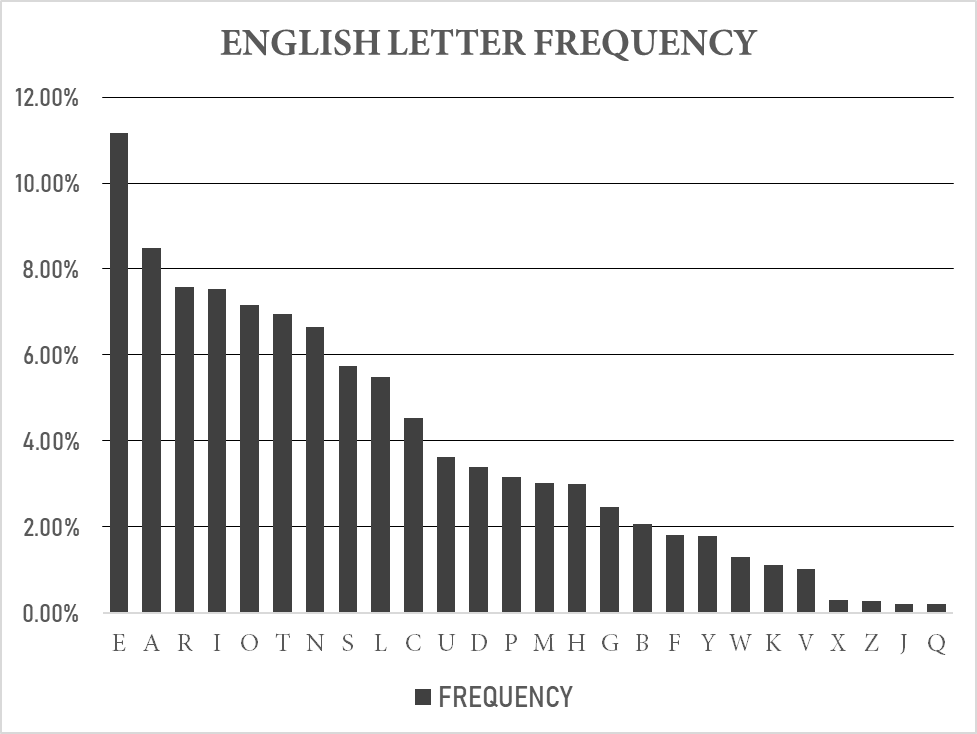
\includegraphics{ENG_FREQ}
\par\end{center}

\medskip{}

We can assume that most samples of text written in English would have
a similar distribution of letters. However this is only true if the
sample of text is long enough. A very short text may lead to a significantly
different distribution.

When trying to decrypt a cipher text based on a substitution cipher,
we can use a frequency analysis to help identify the most recurring
letters in a cipher text and hence make hypothesis of what these letters
have been encoded as (e.g. E, T, A, O, etc.) This will help us decrypt
some of the letters in the text. We can then recognise patterns/words
in the partly decoded text to identify more substitutions.

\subsubsection{Brute Force/Exhaustive Key Search}

In cryptography, a brute-force attack consists of an attacker submitting
many passwords or passphrases with the hope of eventually guessing
a combination correctly. The attacker systematically checks all possible
passwords and passphrases until the correct one is found. Alternatively,
the attacker can attempt to guess the key which is typically created
from the password using a key derivation function. This is known as
an exhaustive key search.

A brute-force attack is a cryptanalytic attack that can, in theory,
be used to attempt to decrypt any encrypted data (except for data
encrypted in an information-theoretically secure manner). Such an
attack might be used when it is not possible to take advantage of
other weaknesses in an encryption system (if any exist) that would
make the task easier

\pagebreak{}

\subsection{Simple Substitution Cipher}

It is an improvement to the Caesar Cipher. Instead of shifting the
alphabets by some number, this scheme uses some permutation of the
letters in alphabet. For example, A, B, $\ldots\:$, Y, Z and Z, Y,
$\ldots\:$, A are two obvious permutation of all the letters in alphabet.
Permutation is nothing but a jumbled up set of alphabets. With 26
letters in alphabet, the possible permutations are 26! (factorial
of 26) which is equal to $4\times10^{26}$. The sender and the receiver
may choose any one of these possible permutation as a ciphertext alphabet.
This permutation is the secret key of the scheme.

\paragraph{Process of Simple Substitution Cipher}
\begin{itemize}
\item Take the alphabets A, B, C,$\ldots\:$, Z in the natural order.
\item The sender and the receiver decide on a randomly selected permutation
of the letters of the alphabet.
\item Underneath the natural order alphabets, write out the chosen permutation
of the letters of the alphabet. For encryption, sender replaces each
plaintext letters by substituting the permutation letter that is directly
beneath it in the table. This process is shown in the following illustration.
In this example, the chosen permutation is given below. The plaintext
\textbf{\textquoteleft EXAMPLE\textquoteright{}} is encrypted to \textbf{\textquoteleft TBQDHST\textquoteright }.
\end{itemize}
\begin{center}
{\footnotesize{}}%
\begin{tabular}{|c|c|c|c|c|c|c|c|c|c|c|c|c|c|c|c|c|c|c|c|c|c|c|c|c|c|c|}
\hline 
{\footnotesize{}$P_t$} & {\footnotesize{}A} & {\footnotesize{}B} & {\footnotesize{}C} & {\footnotesize{}D} & {\footnotesize{}E} & {\footnotesize{}F} & {\footnotesize{}G} & {\footnotesize{}H} & {\footnotesize{}I} & {\footnotesize{}J} & {\footnotesize{}K} & {\footnotesize{}L} & {\footnotesize{}M} & {\footnotesize{}N} & {\footnotesize{}O} & {\footnotesize{}P} & {\footnotesize{}Q} & {\footnotesize{}R} & {\footnotesize{}S} & {\footnotesize{}T} & {\footnotesize{}U} & {\footnotesize{}V} & {\footnotesize{}W} & {\footnotesize{}X} & {\footnotesize{}Y} & {\footnotesize{}Z}\tabularnewline
\hline 
\hline 
{\footnotesize{}$C_t$} & {\footnotesize{}Q} & {\footnotesize{}W} & {\footnotesize{}E} & {\footnotesize{}R} & {\footnotesize{}T} & {\footnotesize{}Y} & {\footnotesize{}U} & {\footnotesize{}I} & {\footnotesize{}O} & {\footnotesize{}P} & {\footnotesize{}A} & {\footnotesize{}S} & {\footnotesize{}D} & {\footnotesize{}F} & {\footnotesize{}G} & {\footnotesize{}H} & {\footnotesize{}J} & {\footnotesize{}K} & {\footnotesize{}L} & {\footnotesize{}Z} & {\footnotesize{}X} & {\footnotesize{}C} & {\footnotesize{}V} & {\footnotesize{}B} & {\footnotesize{}N} & {\footnotesize{}M}\tabularnewline
\hline 
\end{tabular}{\footnotesize\par}
\par\end{center}
\begin{itemize}
\item On receiving the ciphertext, the receiver, who also knows the randomly
chosen permutation, replaces each ciphertext letter on the bottom
row with the corresponding plaintext letter in the top row. The ciphertext
\textbf{\textquoteleft TBQDHST\textquoteright{}} is decrypted to \textbf{\textquoteleft EXAMPLE\textquoteright }.
\end{itemize}

\end{document}
